\documentclass[a4paper]{article}
\usepackage{graphicx}
\usepackage{wrapfig}
\usepackage{caption}
\usepackage{subcaption}


\title{Selection Sort}
\author{Yarne Ramakers}
\date{\today}

\begin{document}

%\maketitle - had to comment as it took up too much space
\begin{center}
  Selection Sort \\
  Yarne Ramakers \\
  \today \\
\end{center}

\begin{figure}[h]
  \begin{subfigure}{0.3\textwidth}
    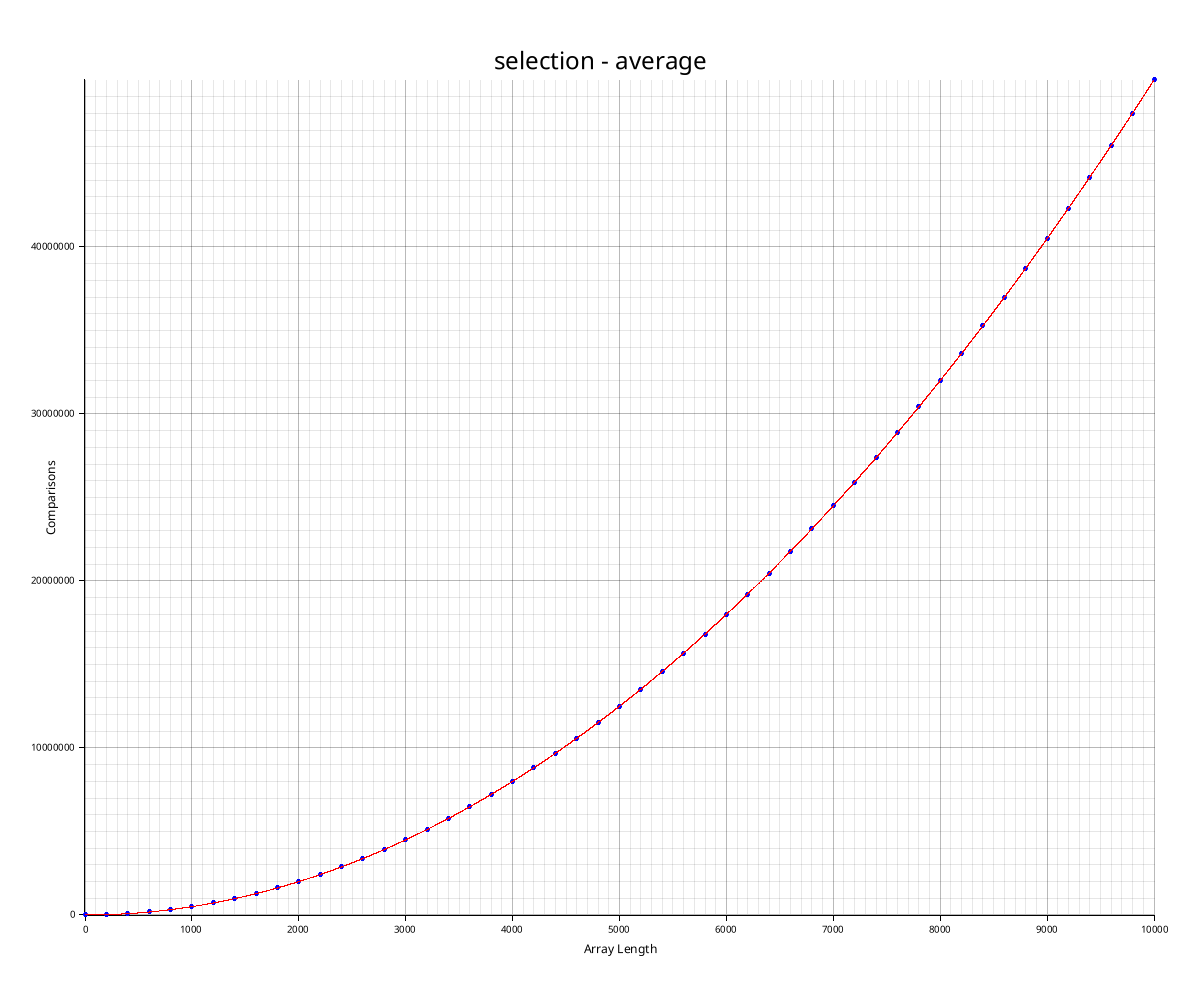
\includegraphics[width=\textwidth]{../plots/selection-average.png}
    \caption{Average case}
    \label{fig:selection-avg}
  \end{subfigure}
  \begin{subfigure}[b]{0.3\textwidth}
    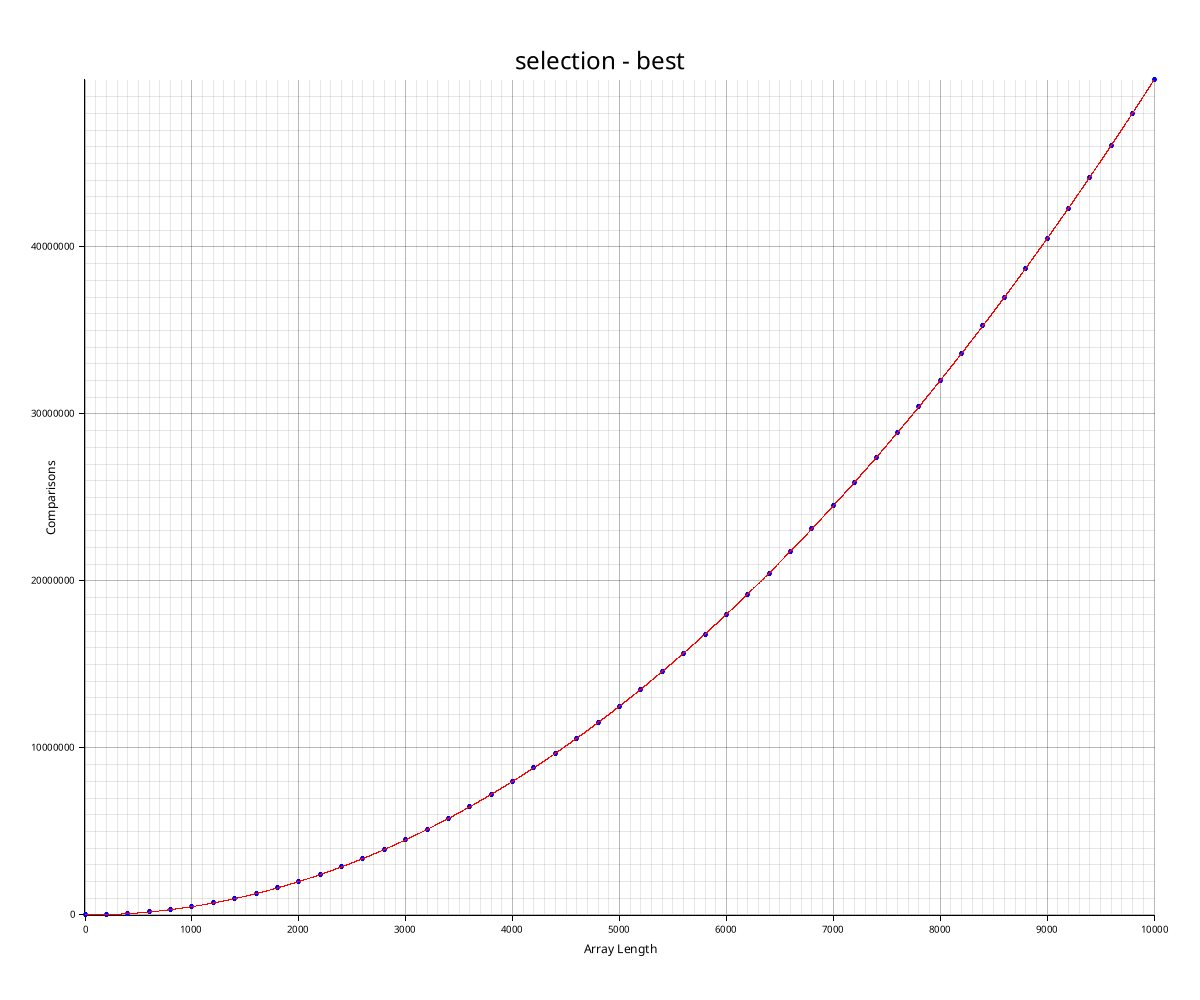
\includegraphics[width=\textwidth]{../plots/selection-best.png}
    \caption{Best case}
    \label{fig:selection-best}
  \end{subfigure}
  \begin{subfigure}[b]{0.3\textwidth}
    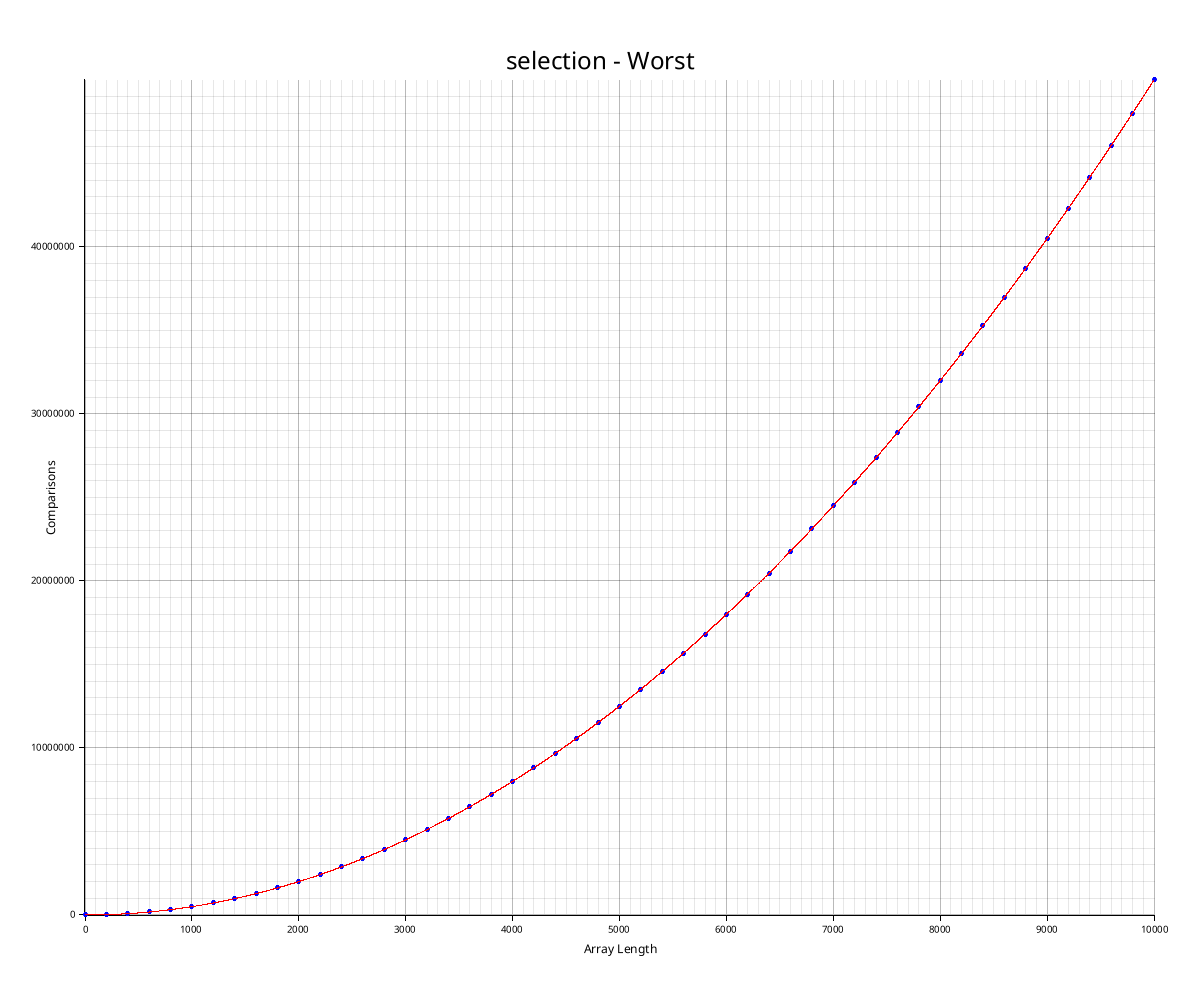
\includegraphics[width=\textwidth]{../plots/selection-worst.png}
    \caption{Worst case}
    \label{fig:selection-worst}
  \end{subfigure}
\end{figure}

\section{Introductie}
% Introduction to selection sort and its importance.

Selection sort is een simpel sorteeralgoritme dat een lijst sorteert door herhaaldelijk het kleinste (of grootste, afhankelijk van de sorteervolgorde en implementatie) element uit de rest van de lijst te selecteren en dit vooraan (of achteraan, afhankelijk van de sorteervolgorde en implementatie) te plaatsen.

\section{Bevindingen}
% Discuss the results of the experiments.
Mijn experimentele bevinding vertonen sterke overeenkomsten met het theoretische model van selection sort.
In de grafiek \ref{fig:selection-avg} toont de rode lijn de theoretische complexiteit van selection sort, namelijk $\sim \frac{1}{2} n^2$. 
De blauwe punten tonen de gemeten vergelijkingen over lijsten voor verschillende lengte $n$. 
Deze $n$ is gekozen tussen 0 en 10 000 met een stapgrootte van 200, per $n$ zijn er ook 5 metingen gebeurd.

\par

Voor lijsten met een kleinere $n$ is de gemeten complexiteit iets kleiner dan de theoretische complexiteit. Dit komt door de overhead van het meten van de complexiteit. Dit is echter niet te zien in de grafiek, omdat de eerste meting bij $n=200$ gebeurt.
En bij $n=200$ zal het verschil tussen het werkelijk aantal vergelijkingen en de theoretische complexiteit maar $100$ vergelijkingen zijn, wat niet zichtbaar is op de grafiek.
Bij kleinere lijsten zullen de kleinere orde termen een grotere invloed hebben op de gemeten complexiteit.
Bij grotere $n$ is de gemeten complexiteit bijna gelijk aan de theoretische complexiteit. 

\par

We maken hier geen onderscheid tussen de beste, slechtste en gemiddelde gevallen. Selection sort zal elke itteratie het kleinste element selecteren en vooraan plaatsen, ongeacht de volgorde van de lijst.
Eerst vergelijken we dus $n-1$ elementen (omdat het te vergelijken element niet vergeleken wordt met zichzelf), in de volgende itteratie $n-2$, daarna $n-3$, enzovoort. Het totaal aantal vergelijkingen in eender welk geval is dan $\sum_{i=1}^{n-1}i \sim \frac{1}{2}n^2$.
Deze bevinding is ook terug te vinden in de grafieken \ref{fig:selection-avg}, \ref{fig:selection-best} en \ref{fig:selection-worst}, het gemiddelde, beste en slechtse geval respectievelijk. Deze grafieken zijn exact hetzelfde, ookal is de best case gemeten op een gesorteerde lijst, de worst case op een omgekeerde gesorteerde lijst en de average case op een willekeurige lijst.

\end{document}